\section{Taking Wavelet Transforms of Inputs}\label{sec:ch6:gainlayer}

In contrast to the previous section where we only parameterized filters in the
wavelet domain and transformed the filters back to the pixel domain to do
convolution, this section explores learning wholly in the wavelet domain. I.e.,
we want to take a wavelet decomposition of the input and learn gains to apply to
these coefficients, and optionally return to the pixel domain.

As neural network training involves presenting thousands of training samples on
memory limited GPUs, we want our layer to be fast and as memory efficient as
possible. To achieve this we would ideally choose to use a critically sampled
filter bank implementation.  The fast 2-D Discrete Wavelet Transform (DWT) is a
possible option, but it has two drawbacks: it has poor directional selectivity
and any alteration of wavelet coefficients will cause the aliasing cancelling
properties of the reconstructed signal to disappear. Another option is to use
the $\DTCWT$ \cite{selesnick_dual-tree_2005}. This comes with a memory overhead
which we discuss more in \autoref{sec:ch6:memory}, but it enables us to have
have better directional selectivity and allows for the possibility of returning
to the pixel domain with minimal aliasing \cite{kingsbury_complex_2001}.

In the next section we describe in more detail how the proposed layer works,
agnostic of the wavelet transform used, before describing the differences between
using the DWT and the $\DTCWT$.
% \subsection{Aliasing in the DWT}
% Consider a single level critically sampled DWT in 1-D. The aliasing cancelling
% condition is:

% $$G_0(z)H_0(-z) + G_1(z)H_1(-z) = 0$$

% This is typically solved by using Quadrature Mirror Filters, i.e.

% \begin{align}
  % H_1(z) &= H_0(-z) \\
  % G_0(z) &= H_0(z) \\
  % G_1(z) &= -H_1(z) = -H_0(-z) 
% \end{align}

\subsection{Background}
As we now want to consider the DWT and the $\DTCWT$ which are both implemented
as filter bank systems, we deviate slightly from the notation in the previous
chapter (which was inspired by sampling a continuous wavelet transform). 

Firstly, instead of talking about the continuous spatial variable $\xy$, we now
consider the discrete spatial variable $\nn = [n_1, n_2]$. We switch to square 
brackets to make this clearer. With the new discrete notation, the output of a CNN at layer $l$ is:
%
\begin{equation}
  \cnndlact{x}{l}{c}{\nn}, \quad c\in \{0, \ldots C_l-1\}, \nn \in \integers[2]
\end{equation}
%
where $c$ indexes the channel dimension. 
We also make use of the 2-D $Z$-transform to simplify our analysis:
%
\begin{equation}
  X(\zz) = \sum_{n_1}\sum_{n_2} x[n_1, n_2]z_1^{-n_1}z_2^{-n_2} =
  \sum_{\nn}x[c, \nn]\zz^{-\nn}
\end{equation}
%
As we are working with three dimensional arrays (two spatial and one channel) but are
only doing convolution in two, we introduce a slightly modified 2-D $Z$-transform
which includes the channel index:
%
\begin{equation}
  X(c, \zz) = \sum_{n_1}\sum_{n_2} x[c, n_1, n_2]z_1^{-n_1}z_2^{-n_2} =
  \sum_{\nn}x[c, \nn]\zz^{-\nn} \label{eq:ch6:ztransform}
\end{equation}

Recall that a typical convolutional
layer in a standard CNN gets the next layer's output in a two-step process:
%
\begin{eqnarray} 
  \cnndlact{y}{l+1}{f}{\nn} &=& \sum_{c=0}^{C_l - 1} \cnndlact{x}{l}{c}{\nn} \conv \cnndfilt{l}{f}{c}{\nn}
    \label{eq:ch6:conv}\\
    \cnndlact{x}{l+1}{f}{\xy} & = & \sigma \left( \cnndlact{y}{l+1}{f}{\xy} \right) \label{eq:ch6:nonlin}
\end{eqnarray}
%
With the new $Z$-transform notation introduced in \eqref{eq:ch6:ztransform}, we
can rewrite \eqref{eq:ch6:conv} as:

\begin{equation}
  \cnnlact{Y}{l+1}{f}{\zz} = \sum_{c=0}^{C_l - 1} \cnnlact{X}{l}{c}{\zz}
  H_f^{(l)}(c, \zz)
\end{equation}
%
Note that we cannot rewrite \eqref{eq:ch6:nonlin} with $Z$-transforms as it is a nonlinear
operation.

Also recall that with multirate systems, upsampling by $M$ takes $X(z)$ to
$X(z^M)$ and downsampling by $M$ takes $X(z)$ to $\frac{1}{M}\sum_{k=0}^{M-1} X(W_M^k
z^{1/k})$ where $W_M^k = e^{\frac{j2\pi k}{M}}$. We will drop the $M$ subscript
below unless it is unclear of the sample rate change, simply using $W^k$.

\section{$\DTCWT$ Single Subband Gain}

\begin{figure}
  \centering
  \begin{tikzpicture}
    \matrix (m1) [minimum height=4mm, column sep=6mm, align=center]
	{
	%--------------------------------------------------------------------
		\node[coordinate]                  (m00) {};    &
		\node[coordinate]                  (m01) {};          &
		\node[dspsquare]                   (m02) {$A(z)$};          &
		\node[circle,draw,inner sep=1pt]   (m03) {\downsamplertext{M}}; &
		\node[dspnodeopen,dsp/label=above] (m04) {$X_a(z)$};          &
		\node[circle,draw,inner sep=1pt]   (m07) {\upsamplertext{M}}; &
		\node[dspsquare]                   (m08) {$C(z)$};          &
		\node[coordinate]                  (m09) {};          &
		\node[coordinate]                  (m0X) {};          \\
		%--------------------------------------------------------------------
		\node[dspnodefull]                 (m10) {};          &
		\node[coordinate]                  (m11) {};          &
		\node[coordinate]                  (m12) {};    &
		\node[coordinate]                  (m13) {};          &
		\node[coordinate]                  (m14) {};    &
		\node[coordinate]                  (m17) {};          &
		\node[coordinate]                  (m18) {};    &
		\node[dspadder]                    (m19) {};          &
		\node[]     (m1X) {};          \\
		%--------------------------------------------------------------------
		\node[coordinate]                  (m20) {};    &
		\node[coordinate]                  (m21) {};          &
		\node[dspsquare]                   (m22) {$B(z)$};          &
		\node[circle,draw,inner sep=1pt]   (m23) {\downsamplertext{M}}; &
		\node[dspnodeopen,dsp/label=below] (m24) {$X_b(z)$};          &
		\node[circle,draw,inner sep=1pt]   (m27) {\upsamplertext{M}}; &
		\node[dspsquare]                   (m28) {$D(z)$};          &
		\node[coordinate]                  (m29) {};          &
		\node[coordinate]                  (m2X) {};          \\
		%--------------------------------------------------------------------
	};
	\draw[dspline] (m10) -- (m11);
	\draw[dspline] (m11) -- (m01);
	\draw[dspline] (m11) -- (m21);
	\foreach \i in {0,2} {
    	\draw[dspconn] (m\i1) -- (m\i2);
    	\draw[dspconn] (m\i2) -- (m\i3);
    	\draw[dspline] (m\i3) -- (m\i4);
    	\draw[dspconn] (m\i4) -- (m\i7);
    	\draw[dspconn] (m\i7) -- (m\i8);
    	\draw[dspline] (m\i8) -- (m\i9);
	}
  \node[left=0pt of m10] (left) {$X(z)$};
  \node[below=9pt of m24] (bottom) {};
  \draw[dspconn] (m09) -- node[right, yshift=5pt] {$Y_a(z)$} (m19);
  \draw[dspconn] (m29) -- node[right, yshift=-5pt] {$Y_b(z)$} (m19);
  \draw[dspconn] (m19) -- node[right, xshift=5pt] {$Y(z)$} (m1X);
	
\end{tikzpicture}

  \mycaption{Block Diagram of 1-D $\DTCWT$}{Note the top and bottom paths are
  through the wavelet or scaling functions from just level m ($M=2^m$). Figure
  based on Figure~4 in \cite{kingsbury_complex_2001}.}
  \label{fig:ch6:dtcwt_two_tree}
\end{figure}

Let us consider one subband of the $\DTCWT$. This includes the coefficients from
both tree A and tree B. For simplicity in this analysis we will consider the 1-D
$\DTCWT$ without the channel parameter $c$. If we only keep coefficients from a given
subband and set all the others to zero, then we have a reduced tree as shown in
\autoref{fig:ch6:dtcwt_two_tree}. The end to end transfer function is:
%
\begin{equation}
  \frac{Y(z)}{X(z)} = \frac{1}{M} \sum_{k=0}^{M-1} \left[A(W^k z)C(z) + B(W^k z)D(z)\right]
  \label{eq:ch6:aliasing}
\end{equation}
%
where the aliasing terms are formed from the addition of the rotated z
transforms, i.e.\ when $k \neq 0$.

\begin{theorem} \label{thm:ch6:shiftinv}
  Suppose we have complex filters $P(z)$ and $Q(z)$ with support only in the
  positive half of the frequency space. If $A(z) = 2\real{P(z)}$, $B(z) =
  2\imag{P(z)}$, $C(z) = 2\real{Q(z)}$ and $D(z) = -2\imag{Q(z)}$, then the aliasing
  terms in \eqref{eq:ch6:aliasing} are nearly zero and the system is nearly
  shift invariant.
\end{theorem}

\begin{proof}
  See section 4 of \cite{kingsbury_complex_2001} for the full proof of
  this, and section 7 for the bounds on what `nearly' shift invariant means. 
  In short, from the definition of $A, B, C$ and $D$ it follows that:  
  \begin{eqnarray*}
    A(z) &=& P(z) + P^*(z) \\
    B(z) &=& -j(P(z) - P^*(z)) \\
    C(z) &=& Q(z) + Q^*(z) \\
    D(z) &=& j(Q(z) - Q^*(z))
  \end{eqnarray*}
  where $H^*(z) = \sum_n h^*[n]z^{-n}$ is the $Z$-transform of the complex
  conjugate of the complex filter $h$. This reflects the purely positive
  frequency support of $P(z)$ to a purely negative one. Substituting these into
  \eqref{eq:ch6:aliasing} gives:
  \begin{equation}
    A(W^k z)C(z) + B(W^k z)D(z) = 2P(W^kz)Q(z) + 2P^*(W^kz)Q^*(z)
    \label{eq:ch6:complex_filts}
  \end{equation}
 Using \eqref{eq:ch6:complex_filts}, Kingsbury shows that it is easier to design
 single side band filters so $P(W^kz)$ does not overlap with $Q(z)$ and
 $P^*(W^kz)$ does not overlap with $Q^*(z)$ for $k \neq 0$.
\end{proof}

Using \autoref{thm:ch6:shiftinv} \eqref{eq:ch6:aliasing} reduces to:
\begin{equation}
 \frac{Y(z)}{X(z)} = \frac{1}{M}\left[ A(z)C(z) + B(z)D(z) \right]
  \label{eq:ch6:aliasing_cancel}
\end{equation}

Let us extend this idea to allow for any linear gain applied to the passbands
(not just zeros and ones). Ultimately, we may want to allow for nonlinear
operations applied to the wavelet coefficients, but we initially restrict
ourselves to linear gains so that we can build from a sensible base. In
particular, if we want to have gains applied to the wavelet coefficients, it
would be nice to maintain the shift invariant properties of the $\DTCWT$.

\begin{figure}
  \centering
  \begin{tikzpicture}
    \matrix (m1) [row sep=5mm, column sep=6mm,align=center,anchor=center]
	{
	%--------------------------------------------------------------------
		\node[coordinate]                  (m00) {};    &
		\node[coordinate]                  (m01) {};          &
		\node[dspsquare]                   (m02) {$A(z)$};          &
		\node[circle,draw,inner sep=1pt]   (m03) {\downsamplertext{M}}; &
		\node[dspnodeopen,dsp/label=above] (m04) {$U_a(z)$};          &
    \node[rectangle,draw,inner sep=2pt](m05) {$G_{aa}(z)$}; &
		\node[dspnodeopen,dsp/label=above] (m06) {$V_a(z)$};          &
		\node[circle,draw,inner sep=1pt]   (m07) {\upsamplertext{M}}; &
		\node[dspsquare]                   (m08) {$C(z)$};          &
		\node[coordinate]                  (m09) {};          &
		\node[coordinate]                  (m0X) {};          \\
		%--------------------------------------------------------------------
      \node[dspnodefull]                 (m10) {};          &
		\node[coordinate]                  (m11) {};          &
		\node[coordinate]                  (m12) {};    &
		\node[coordinate]                  (m13) {};          &
		\node[coordinate]                  (m14) {};    &
		\node[coordinate]                  (m15) {};          &
		\node[coordinate]                  (m16) {};    &
		\node[coordinate]                  (m17) {};          &
		\node[coordinate]                  (m18) {};    &
		\node[dspadder]                    (m19) {};          &
    \node[]                            (m1X) {$Y(z)$};          \\
		%--------------------------------------------------------------------
		\node[coordinate]                  (m20) {};    &
		\node[coordinate]                  (m21) {};          &
		\node[dspsquare]                   (m22) {$B(z)$};          &
		\node[circle,draw,inner sep=1pt]   (m23) {\downsamplertext{M}}; &
		\node[dspnodeopen,dsp/label=below] (m24) {$U_b(z)$};          &
      \node[rectangle,draw,inner sep=2pt](m25) {$G_{bb}(z)$}; &
		\node[dspnodeopen,dsp/label=below] (m26) {$V_b(z)$};          &
		\node[circle,draw,inner sep=1pt]   (m27) {\upsamplertext{M}}; &
		\node[dspsquare]                   (m28) {$D(z)$};          &
		\node[coordinate]                  (m29) {};          &
		\node[coordinate]                  (m2X) {};          \\
		%--------------------------------------------------------------------
  };
	\draw[dspline] (m10) -- (m11);
	\draw[dspline] (m11) -- (m01);
	\draw[dspline] (m11) -- (m21);
	\foreach \i in {0,2} {
    	\draw[dspconn] (m\i1) -- (m\i2);
    	\draw[dspconn] (m\i2) -- (m\i3);
    	\draw[dspline] (m\i3) -- (m\i4);
    	\draw[dspconn] (m\i4) -- (m\i5);
    	\draw[dspline] (m\i5) -- (m\i6);
    	\draw[dspconn] (m\i6) -- (m\i7);
    	\draw[dspconn] (m\i7) -- (m\i8);
    	\draw[dspline] (m\i8) -- (m\i9);
	}
	%\draw[dspflow] (m04) --  (m06);
	%\draw[dspflow] (m24) -- (m26);
  \draw[dspconn] (m24) -- node[draw,pos=0.7,inner sep=2pt,fill=white] {$G_{ba}(z)$} (m06);
  \draw[dspconn] (m04) -- node[draw,pos=0.7,inner sep=2pt,fill=white] {$G_{ab}(z)$} (m26);
  \draw[dspconn] (m09) -- node[right] {$Y_a(z)$} (m19);
  \draw[dspconn] (m29) -- node[right] {$Y_b(z)$} (m19);
	\draw[dspconn] (m19) -- (m1X);
  \node[left=0pt of m10] (left) {$X(z)$};
  \node[below=10pt of m24] (bottom) {};
	
\end{tikzpicture}

  \mycaption{Block Diagram of 1-D $\DTCWT$}{Note the top and bottom paths are
  through the wavelet or scaling functions from just level m ($M=2^m$). Figure
  based on Figure~4 in \cite{kingsbury_complex_2001}.}
  \label{fig:ch6:dtcwt_two_tree_gain}
\end{figure}

\autoref{fig:ch6:dtcwt_two_tree_gain} shows a block diagram of the extension of 
the above to general gains. This is a two port network with four individual
transfer functions. Let the transfer fucntion from $U_i$ to $V_j$
be $G_{ij}$ for $i, j \in \{a, b\}$. Then $V_a$ and $V_b$ are:
\begin{eqnarray}
  V_a(z) &=& U_a(z)G_{aa}(z) + U_b(z)G_{ba}(z) \\
         &=& \frac{1}{M} \sum_k X(W^{k} z^{1/k}) \left[A(W^k z^{1/k})G_{aa}(z) +
             B(W^k z^{1/k}) G_{ba}(z) \right] \\
  V_b(z) &=& U_a(z)G_{ab}(z) + U_b(z)G_{bb}(z) \\
         &=& \frac{1}{M} \sum_k X(W^{k} z^{1/k}) \left[A(W^k z^{1/k})G_{ab}(z) +
             B(W^k z^{1/k}) G_{bb}(z) \right] 
\end{eqnarray}
%
Further, $Y_a$ and $Y_b$ are:
\begin{eqnarray}
  Y_a(z) &=& C(z)V_a(z^M) \\
  Y_b(z) &=& D(z)V_b(z^M)
\end{eqnarray}
%
Then the end to end transfer function is:
\begin{equation}
  \begin{split}
  % \begin{multline}
    Y(z) = Y_{a}(z) + Y_{b}(z) = \frac{1}{M} \sum_{k=0}^{M-1} X(W^k z)
    & \left[  A(W^kz)C(z)G_{aa}(z^k) + B(W^kz)D(z)G_{bb}(z) + \right. \\
    & \left. \hphantom{[}  B(W^kz)C(z)G_{ba}(z^k) + A(W^kz)D(z)G_{ba}(z) \right] 
    \label{eq:ch6:transfer}
  % \end{multline}
  \end{split}
\end{equation}

\begin{theorem}\label{thm:ch6:shiftinvgain}
  If we let $G_{aa}(z^k) = G_{bb}(z^k) = G_r(z^k)$ and $G_{ab}(z^k) = -G_{ba}(z^k) = G_i(z^k)$
  then the end to end transfer function is shift invariant.
\end{theorem}
\begin{proof}
  Using the above substitutions, the terms in the square brackets of
  \eqref{eq:ch6:transfer} become:
  \begin{equation}\label{eq:ch6:realimag}
    G_r(z^k)\left[A(W^kz)C(z) + B(W^kz)D(z)\right] + G_i(z^k)\left[A(W^kz)D(z) - B(W^kz)C(z)\right]
  \end{equation}
  \autoref{thm:ch6:shiftinv} already showed that the $G_r$ terms are shift
  invariant and reduce to $A(z)C(z) + B(z)D(z)$. To prove the same for the $G_i$
  terms, we follow the same procedure. Using our definitions of $A, B, C, D$
  from \autoref{thm:ch6:shiftinv} we note that:
  %
  \begin{eqnarray}
    A(W^kz)D(z) - B(W^kz)C(z) &=& j\left[P(W^kz) + P^*(W^kz)\right]\left[Q(z) -Q^*(z)\right] +\\
                              &&j\left[P(W^kz) -P^*(W^kz)\right]\left[Q(z) + Q^*(z)\right] \\
                              &=& 2j\left[P(W^kz)Q(z) - P^*(W^kz)Q^*(z)\right]
  \end{eqnarray}
  We note that the difference
  between the $G_r$ and $G_i$ terms is just in the sign of the negative
  frequency parts, $AD - BC$ is the Hilbert pair of $AC+BD$. To prove shift
  invariance for the $G_r$ terms in \autoref{thm:ch6:shiftinv}, we ensured that
  $P(W^kz)Q(z) \approx 0$ and $P^*(W^kz)Q^*(z) \approx 0$ for $k\neq 0$. We can
  use this again here to prove the shift invariance of the $G_i$ terms in
  \eqref{eq:ch6:realimag}. This completes our proof.
\end{proof}

Using \autoref{thm:ch6:shiftinvgain}, the end to end transfer function with the
gains is now
\begin{eqnarray}
  \frac{Y(z)}{X(z)} &=& \frac{2}{M} \left[G_r(z^{M}) \left(A(z)C(z) + B(z)D(z)\right)
  + G_i(z^{M}) \left(A(z)D(z) - B(z)C(z)\right) \right] \\
  &=& \frac{2}{M}\left[G_r(z^{M}) \left(PQ + P^*Q^*\right)
  + jG_i(z^{M}) \left(PQ - P^*Q^*\right) \right]  \label{eq:ch6:end2end}
\end{eqnarray}

Now we know can assume that our $\DTCWT$ is well designed and extracts frequency
bands at local areas, then our complex filter $G(z)=G_r(z) + jG_i(z)$ allows us
to modify these passbands (e.g.\ by simply scaling if $G(z) = C$, or by more
complex functions.


\subsection{Backpropagation Analysis}
We start with the commonly known property that for a convolutional block, the
gradient with respect to the input is the gradient with respect to the output
convolved with the time reverse of the filter. More formally, if 
$Y(z) = H(z) X(z)$:
%
\begin{equation}\label{eq:ch6:backprop}
  \Delta X(z) = H(z^{-1}) \Delta Y(z)
\end{equation}
%
where $H(z^{-1})$ is the $Z$-transform of the time/space reverse of $H(z)$,
$\Delta Y(z) \triangleq \dydx{L}{Y}(z)$ is the gradient of the loss with respect
to the output, and $\Delta X(z) \triangleq \dydx{L}{X}(z)$ is the gradient of
the loss with respect to the input. If H were complex, the first term in
\autoref{eq:ch6:backprop} would be $\bar{H}(1/\bar{z})$, but as each individual
block in the $\DTCWT$ is purely real, we can use the simpler form. 

Assume we already have access to the quantity $\Delta Y(z)$ (this is the input
to the backwards pass). \autoref{fig:ch6:bwd_pass} illustrates the
backpropagation procedure. An interesting result is that the backwards pass of
an inverse wavelet transform is equivalent to doing a forward wavelet
transform.\footnote{As shown in \autoref{fig:ch6:bwd_pass}, the analysis and
synthesis filters have to be swapped and time reversed. For orthogonal wavelet
transforms, the synthesis filters are already the time reverse of the analysis
filters, so no change has to be done. The q-shift filters of the $\DTCWT$
\cite{kingsbury_design_2003} have this property.} Similarly, the backwards pass
of the forward transform is equivalent to doing the inverse transform. The
weight update gradients are then calculated by finding 
\textbf{FIX this - make it not use the $\DTCWT$ to get delta v}.
$\Delta V(z) = \DTCWT\left\{ \Delta Y(z) \right\}$ and then convolving with the 
time reverse of the saved wavelet coefficients from the forward pass - $U(z)$.

\begin{gather}
  \Delta G_r(z) = \Delta V_r(z) U_r(z^{-1}) + \Delta V_i(z) U_i(z^{-1})  \label{eq:ch6:gr_update}\\
  \Delta G_i(z) =  -\Delta V_r(z) U_i(z^{-1}) + \Delta V_i(z) U_r(z^{-1})  \label{eq:ch6:gi_update} 
\end{gather}

Unsurprisingly, the passthrough gradients have similar form to
\autoref{eq:ch6:end2end}:
\begin{equation}\label{eq:ch6:passthrough}
    \Delta X(z) = \frac{2\Delta Y(z)}{M} \left[G_r(z^{-M})\left( PQ + P^*Q^* \right)\right. + 
      \left. jG_i(z^{-M}) \left(PQ-P^*Q^* \right) \right] 
\end{equation}
where we have dropped the $z$ terms on $P(z), Q(z), P^*(z), Q^*(z)$ for brevity.

Note that we only need to evaluate equations
~\ref{eq:ch6:gr_update},\ref{eq:ch6:gi_update},\ref{eq:ch6:passthrough} over the
support of $G(z)$ i.e., if it is a single number we only need to calculate
$\left.\Delta G(z)\right\rvert_{z=0}$.

\begin{figure}[ht]
  \centering
  % \subfloat[]{%
    % 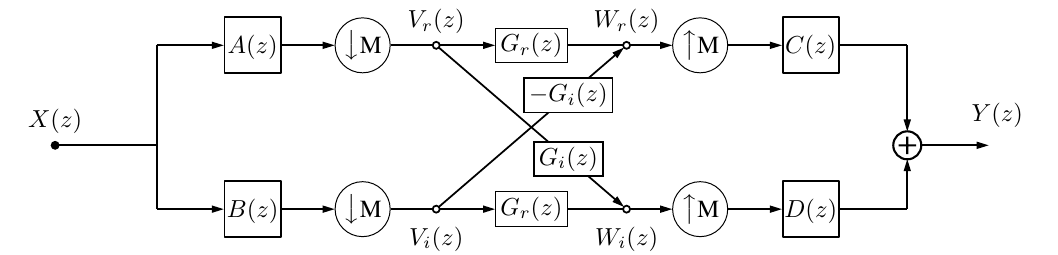
\includegraphics[width=.85\textwidth]{freqlearn/images/top_block.png}
    % \label{fig:ch6:fwd_pass}
  % }
   % \newline
  % \subfloat[]{%
    % 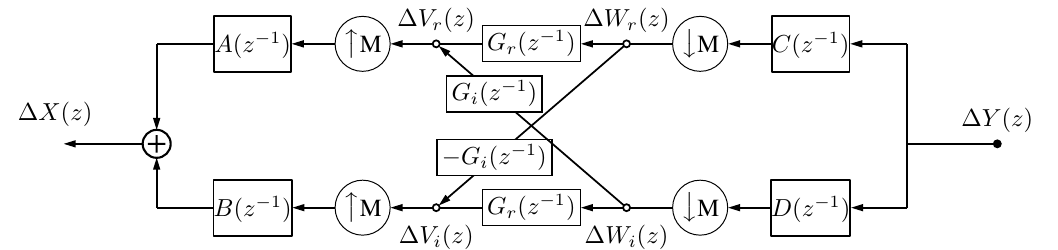
\includegraphics[width=.85\textwidth]{freqlearn/images/bottom_block.png}
    % \label{fig:ch6:bwd_pass}
  % }
  \makebox[\textwidth][c]{%
    \resizebox{1.1\textwidth}{!}{\begin{tikzpicture}
    \matrix (m1) [row sep=5mm, column sep=6mm,align=center,anchor=center]
	{
	% %--------------------------------------------------------------------
		% \node[coordinate]                  (m00) {};    &
		% \node[coordinate]                  (m01) {};          &
		% \node[dspsquare]                   (m02) {$A(z)$};          &
		% \node[circle,draw,inner sep=1pt]   (m03) {\downsamplertext{M}}; &
		% \node[dspnodeopen,dsp/label=above] (m04) {$V_r(z)$};          &
		% \node[rectangle,draw,inner sep=2pt](m05) {$G_r(z)$}; &
		% \node[dspnodeopen,dsp/label=above] (m06) {$W_r(z)$};          &
		% \node[circle,draw,inner sep=1pt]   (m07) {\upsamplertext{M}}; &
		% \node[dspsquare]                   (m08) {$C(z)$};          &
		% \node[coordinate]                  (m09) {};          &
		% \node[coordinate]                  (m0X) {};          \\
		% %--------------------------------------------------------------------
		% \node[]                            (m10) {$X(z)$};          &
		% \node[coordinate]                  (m11) {};          &
		% \node[coordinate]                  (m12) {};    &
		% \node[coordinate]                  (m13) {};          &
		% \node[coordinate]                  (m14) {};    &
		% \node[coordinate]                  (m15) {};          &
		% \node[coordinate]                  (m16) {};    &
		% \node[coordinate]                  (m17) {};          &
		% \node[coordinate]                  (m18) {};    &
		% \node[dspadder]                    (m19) {};          &
    % \node[]                            (m1X) {$Y(z)$};          \\
		% %--------------------------------------------------------------------
		% \node[coordinate]                  (m20) {};    &
		% \node[coordinate]                  (m21) {};          &
		% \node[dspsquare]                   (m22) {$B(z)$};          &
		% \node[circle,draw,inner sep=1pt]   (m23) {\downsamplertext{M}}; &
		% \node[dspnodeopen,dsp/label=below] (m24) {$V_i(z)$};          &
		% \node[rectangle,draw,inner sep=2pt](m25) {$G_r(z)$}; &
		% \node[dspnodeopen,dsp/label=below] (m26) {$W_i(z)$};          &
		% \node[circle,draw,inner sep=1pt]   (m27) {\upsamplertext{M}}; &
		% \node[dspsquare]                   (m28) {$D(z)$};          &
		% \node[coordinate]                  (m29) {};          &
		% \node[coordinate]                  (m2X) {};          \\
		% %--------------------------------------------------------------------
		% &&&&&&&&& \\
		\node[coordinate]                  (m00a) {};    &
		\node[coordinate]                  (m01a) {};          &
		\node[dspsquare]                   (m02a) {$A\left(z^{-1}\right)$};          &
		\node[circle,draw,inner sep=1pt]   (m03a) {\upsamplertext{M}}; &
		\node[dspnodeopen,dsp/label=above] (m04a) {$\Delta U_r(z)$};          &
		%\node[coordinate]                  (m05) {}; &
		\node[rectangle,draw,inner sep=2pt](m05a) {$G_r\left(z^{-1}\right)$}; &
		\node[dspnodeopen,dsp/label=above] (m06a) {$\Delta V_r(z)$};          &
		\node[circle,draw,inner sep=1pt]   (m07a) {\downsamplertext{M}}; &
		\node[dspsquare]                   (m08a) {$C\left(z^{-1}\right)$};          &
		\node[coordinate]                  (m09a) {};          &
		\node[coordinate]                  (m0Xa) {};          \\
		%--------------------------------------------------------------------
		%\node[coordinate]  (m10) {$\Delta X(z)$};          &
    \node[]                            (m10a) {$\Delta X(z)$}; &
		\node[dspadder]                    (m11a) {};          &
		\node[coordinate]                  (m12a) {};    &
		\node[coordinate]                  (m13a) {};          &
		\node[coordinate]                  (m14a) {};    &
		\node[coordinate]                  (m15a) {};          &
		\node[coordinate]                  (m16a) {};    &
		\node[coordinate]                  (m17a) {};          &
		\node[coordinate]                  (m18a) {};    &
		\node[coordinate]                  (m19a) {};          &
		\node[]                            (m1Xa) {$\Delta Y(z)$};          \\
		%--------------------------------------------------------------------
		\node[coordinate]                  (m20a) {};    &
		\node[coordinate]                  (m21a) {};          &
		\node[dspsquare]                   (m22a) {$B\left(z^{-1}\right)$};          &
		\node[circle,draw,inner sep=1pt]   (m23a) {\upsamplertext{M}}; &
		\node[dspnodeopen,dsp/label=below] (m24a) {$\Delta U_i(z)$};          &
		%\node[coordinate]                  (m25) {}; &
		\node[rectangle,draw,inner sep=2pt](m25a) {$G_r\left(z^{-1}\right)$}; &
		\node[dspnodeopen,dsp/label=below] (m26a) {$\Delta V_i(z)$};          &
		\node[circle,draw,inner sep=1pt]   (m27a) {\downsamplertext{M}}; &
		\node[dspsquare]                   (m28a) {$D\left(z^{-1}\right)$};          &
		\node[coordinate]                  (m29a) {};          &
		\node[coordinate]                  (m2Xa) {};          \\
		%--------------------------------------------------------------------
	};
	% \draw[dspline] (m10) -- (m11);
	% \draw[dspline] (m11) -- (m01);
	% \draw[dspline] (m11) -- (m21);
	% \foreach \i in {0,2} {
      % \draw[dspconn] (m\i1) -- (m\i2);
      % \draw[dspconn] (m\i2) -- (m\i3);
      % \draw[dspline] (m\i3) -- (m\i4);
      % \draw[dspconn] (m\i4) -- (m\i5);
      % \draw[dspline] (m\i5) -- (m\i6);
      % \draw[dspconn] (m\i6) -- (m\i7);
      % \draw[dspconn] (m\i7) -- (m\i8);
      % \draw[dspline] (m\i8) -- (m\i9);
	% }
	% %\draw[dspflow] (m04) --  (m06);
	% %\draw[dspflow] (m24) -- (m26);
	% \draw[dspconn] (m24) -- node[draw,pos=0.7,inner sep=2pt,fill=white] {$-G_i(z)$} (m06);
	% \draw[dspconn] (m04) -- node[draw,pos=0.7,inner sep=2pt,fill=white] {$G_i(z)$} (m26);
	% \draw[dspconn] (m09) -- (m19);
	% \draw[dspconn] (m29) -- (m19);
	% \draw[dspconn] (m19) -- (m1X);
	\draw[dspconn] (m11a) -- (m10a);
	\draw[dspconn] (m01a) -- (m11a);
	\draw[dspconn] (m21a) -- (m11a);
	\foreach \i in {0,2} {
    	\draw[dspconn] (m\i9a) -- (m\i8a);
    	\draw[dspconn] (m\i8a) -- (m\i7a);
    	\draw[dspline] (m\i7a) -- (m\i6a);
    	\draw[dspconn] (m\i6a) -- (m\i5a);
    	\draw[dspline] (m\i5a) -- (m\i4a);
    	\draw[dspconn] (m\i4a) -- (m\i3a);
    	\draw[dspconn] (m\i3a) -- (m\i2a);
    	\draw[dspline] (m\i2a) -- (m\i1a);
	}
	%\draw[dspflow] (m04) --  (m06);
	%\draw[dspflow] (m24) -- (m26);
	\draw[dspconn] (m06a) -- node[draw,pos=0.7,inner sep=2pt,fill=white] {$-G_i\left(z^{-1}\right)$} (m24a);
	\draw[dspconn] (m26a) -- node[draw,pos=0.7,inner sep=2pt,fill=white] {$G_i\left(z^{-1}\right)$} (m04a);
	\draw[dspline] (m09a) -- (m19a);
	\draw[dspline] (m29a) -- (m19a);
	\draw[dspline] (m19a) -- (m1Xa);
	
\end{tikzpicture}
}
  }
  \mycaption{Forward and backward block diagrams for $\DTCWT$ gain layer}{Based
    on Figure~4 in \cite{kingsbury_complex_2001}. Ignoring the $G$ gains, the
    top and bottom paths (through $A, C$ and $B, D$ respectively) make up the
    the real and imaginary parts for \emph{one subband} of the dual tree system.
    Combined, $A+jB$ and $C-jD$ make the complex filters necessary to have
    support on one side of the Fourier domain (see
    \autoref{fig:ch6:dtcwt_bands}). Adding in the complex gain $G_r + jG_i$, we
    can now attenuate/shape the impulse response in each of the subbands. To
    allow for learning, we need backpropagation. The bottom diagram indicates
    how to pass gradients $\Delta Y(z)$ through the layer. Note that upsampling
    has become downsampling, and convolution has become convolution with the
  time reverse of the filter (represented by $z^{-1}$ terms).}
  \label{fig:ch6:fwd_bwd}
\end{figure}




\section{$\DTCWT$ Multiple Subband Gains}\label{sec:ch6:multiple_subbands}

Now that we have the framework for applying a complex gain at one subband, we
can extend this to all of the subbands in the $\DTCWT$. We also reintroduce the channel
dimension. 

In 2-D, a $J$ scale $\DTCWT$ gives $6J+1$ coefficients, 6 sets of complex
coefficients for each scale (representing the oriented bands from 15 to 165
degrees) and 1 set of real lowpass coefficients. Let us write this as:

\begin{equation}
  \DTCWT\{x\} = \{u_{lp}, u_{j,k} \}_{1\leq j\leq J, 1\leq k\leq 6}
  \label{eq:ch6:wave_coeffs}
\end{equation}
%
Sometimes we may want to refer to all of the subband coefficients at a single scale
with one variable, in which case we will call them $\vec{u}_{j}$.

To do the mixing across the $C_l$ channels at each subband, giving $C_{l+1}$
output channels, we introduce the learnable filters:
%
\begin{eqnarray}
  g_{lp} &\in& \reals[C_{l+1}\x C_l\x k_h\x k_w] \label{eq:ch6:glp} \\
  g_{1,1} &\in& \complexes[C_{l+1}\x C_l\x k_h\x k_w] \\
  g_{1,2} &\in& \complexes[C_{l+1}\x C_l\x k_h\x k_w] \\
      & \vdots &\\
  g_{J,6} &\in& \complexes[C_{l+1}\x C_l\x k_h\x k_w]  \label{eq:ch6:gj6}
\end{eqnarray}
%
where $k_h, k_w$ are the sizes of the mixing kernels. These could be $1\x 1$ for
simple gain control, or could be larger, say $3\x 3$, to do more complex
filtering on the subbands. Let us index the lowpass filters $g_{lp}$ and the
bandpass filters $g_{j,k}$ as $g_{lp}[f, c, \nn]$ and $g_{j,k}[f, c, \nn]$.

With these gains we create new coefficients:
\begin{eqnarray}
  v_{lp}[f, \nn] &= & \sum_{c=0}^{C_l-1} u_{lp}[c, \nn] \conv g_{lp}[f, c, \nn] \\
  v_{1,1}[f, \nn] &= & \sum_{c=0}^{C_l-1} u_{1,1}[c, \nn] \conv g_{1,1}[f, c, \nn] \\
  v_{1,2}[f, \nn] &= & \sum_{c=0}^{C_l-1} u_{1,2}[c, \nn] \conv g_{1,2}[f, c, \nn] \\
                  & \vdots & \\
  v_{J,6}[f, \nn] &= & \sum_{c=0}^{C_l-1} u_{J,6}[c, \nn] \conv g_{J,6}[f, c, \nn] 
\end{eqnarray}

I.e., we do independent mixing at each of the different subbands. For $1\x 1$
kernels, this is simply a matrix multiply of the wavelet coefficients. Note that
for complex signals $a, b$ the convolution $a \conv b$ is defined as $(a_r \conv
b_r - a_i \conv b_i) + j(a_r \conv b_i + a_i \conv b_r)$.


\subsection{Examples}
\autoref{fig:ch6:dtcwt_bands} show example impulse responses of our layer.
These impulses were generated by randomly initializing both the real and
imaginary parts of $g_{2,k} \in \complexes[1\x 1]$ from $\mathcal{N}(0,1)$
independently for the six orientations $k$. $g_{1,k}, g_{lp}$ are set to 0. 
I.e. each shape has 12 random variables. It is good
to see that there is still a large degree of variability between shapes. Our
experiments have shown that the distribution of the normalized cross-correlation
between 512 of such randomly generated shapes matches the distribution for
random vectors with roughly 11.5 degrees of freedom.
\autoref{fig:ch6:dtcwt_bands} shows the frequency support of the $6J+1$ subbands
for a two scale $\DTCWT$ as well as some of the equivalent impulse responses for
a randomly initialized set of $g$ filters.

\begin{tikzpicture}[%
  path image/.style={
    path picture={
      \node at (path picture bounding box.center) {
        \includegraphics[height=2.0cm]{#1}
      };
    }
  }, 
  path pic/.style={
    path picture={
      \node at (path picture bounding box.center) {
        \includegraphics[height=1.2cm]{#1}
      };
    }
  }, 
  path pic2/.style={
    path picture={
      \node at (path picture bounding box.center) {
        \includegraphics[height=0.8cm]{#1}
      };
    }
  }, 
  scale=0.6]

  \tikzcuboid{
  shiftx=-1.5cm,
  shifty=-2.5cm,
  scale=0.5,
  anglex=0, 
  angley=90, 
  anglez=230,
  dimx=3, 
  dimy=3, 
  dimz=6,
  densityx=1, 
  densityy=1, 
  densityz=1,
  shade=false,
  emphedge=true,
  shadeopacity=0,
  emphstyle/.style={rounded corners=0.2pt,line width=0.3mm},
  front/.style={draw=blue!50!white,fill=blue!50!white},%
  right/.style={draw=blue!50!white,fill=blue!50!white},%
  top/.style={draw=blue!50!white,fill=blue!50!white},%
  drawxdims=true,
  dimxval=W,
  drawydims=true,
  dimyval=H,
  drawzdims=true,
  dimzval=C_l,
  }
  \draw (0, .3, 0) node {\large{$x^{(l)}$}};
  \draw [path image=\imgpath/waveys.png, draw=black] (1.5,1.5,0) rectangle (6,0,0);
  \draw (3.75, 1.9, 0) node {\large{$\psi_{j, \theta}$}};
  \draw (1.5,0,0) -- (3,-1.7,0);
  \draw (6,0,0) -- (3.3,-1.7,0);
  \draw [path pic2=\imgpath/lowpass.png, draw=black] (2.5,-2.5,10) rectangle (3.5,-1.5,10);
  \draw (3, -1.1, 10) node {\large{$\phi_{j}$}};
  \draw (3.5,-1.5,10) -- (3.5,-1.7,8);

  % \draw (2.4, -1.5, 0) node {\Large{$\conv$}};
  \draw (2.5, -1.5, 3) node {\Large{$\conv$}};
  \draw [->, fill=gray!30,ultra thick] (4, -1.5, 0) -- (5, -1.5, 0);
  \draw [->, fill=gray!30,ultra thick] (4.5, -1.5, 9) -- (5.85, -1.5, 11);

  \tikzcuboid{
  shiftx=3cm,
  shifty=-1.7cm,
  shiftz=0,
  scale=0.3,
  dimx=1, dimy=1, dimz=4,
  densityx=2, densityy=2, densityz=2,
  drawxdims=false,
  drawydims=false,
  drawzdims=true,
  dimzval=12,
  front/.style={draw=yellow!70!white,fill=yellow!70!white},%
  right/.style={draw=yellow!70!white,fill=yellow!70!white},%
  top/.style={draw=yellow!70!white,fill=yellow!70!white},%
  }
  \tikzcuboid{
  shiftz=8/0.3,
  scale=0.3,
  dimx=1, dimy=1, dimz=1,
  densityx=2, densityy=2, densityz=2,
  drawxdims=false,
  drawydims=false,
  drawzdims=false,
  }


  \tikzcuboid{
  shiftx=6cm,
  shifty=-2.0cm,
  shiftz=0.8cm,
  scale=0.5,
  dimx=2, dimy=2, dimz=4,
  densityx=4, densityy=4, densityz=2,
  drawzdims=true,
  dimzval=C_l,
  front/.style={draw=blue!50!white,fill=blue!50!white},%
  right/.style={draw=blue!50!white,fill=blue!50!white},%
  top/.style={draw=blue!50!white,fill=blue!50!white},%
  }

  \tikzcuboid{
  shiftx=6cm,
  shifty=-2cm,
  shiftz=0cm,
  scale=0.5,
  dimx=2, dimy=2, dimz=24,
  densityx=2, densityy=2, densityz=2,
  drawxdims=true,
  dimxval=\frac{W}{2},
  drawydims=true,
  dimyval=\frac{H}{2},
  drawzdims=true,
  dimzval=12C_l,
  front/.style={draw=blue!50!white,fill=blue!50!white},%
  right/.style={draw=blue!50!white,fill=blue!50!white},%
  top/.style={draw=blue!50!white,fill=blue!50!white},%
  }

  % \draw [->, fill=gray!30,ultra thick] (8.5, -1.5, 0) -- (10.5, -1.5, 0) node[midway, above] (mag) {\large{$\lvert\cdot\rvert$}};
  \draw [->, fill=gray!30,ultra thick] (8.5, -1.5, 0) -- (10.5, -1.5, 0) node[midway, above] (mag) {\Large{ $\lvert \cdot \rvert$} };
  \draw [path pic=\imgpath/mag.png, draw=white] (9.25,0,0) rectangle (11.75,2,0);
  \draw (9.25,0,0) -- (mag.north);
  \draw (11.75,0,0) -- (mag.north);
  \draw[->, fill=gray!30, ultra thick] (8.5, -2, 10) -- (10, -3, 3);

  \tikzcuboid{
  shiftx=11.5cm,
  shifty=-2cm,
  scale=0.5,
  dimx=2, dimy=2, dimz=12,
  densityx=2, densityy=2, densityz=2,
  dimzval=6C_l,
  drawxdims=false,
  drawydims=false,
  front/.style={draw=blue!50!white,fill=blue!50!white},%
  right/.style={draw=blue!50!white,fill=blue!50!white},%
  top/.style={draw=blue!50!white,fill=blue!50!white},%
  }
  \tikzcuboid{
  shiftx=11.5cm,
  shifty=-2cm,
  shiftz=8,
  scale=0.5,
  drawxdims=true,
  drawydims=true,
  dimx=2, dimy=2, dimz=4,
  densityx=2, densityy=2, densityz=2,
  dimzval=C_l,
  front/.style={draw=blue!50!white,fill=blue!50!white},%
  right/.style={draw=blue!50!white,fill=blue!50!white},%
  top/.style={draw=blue!50!white,fill=blue!50!white},%
  }
  \draw (13.2, 0.8, 0) node {\large{$z^{(l+1)}$}};
  \draw (20.5, 0.3, 0) node {\large{$y^{(l+1)}$}};
  \draw (24.5, 0.3, 0) node {\large{$x^{(l+1)}$}};
  \draw (14, -1.5, 0) node {\Large{$\conv$}};

  \tikzcuboid{
  shiftx=15.2cm,
  shifty=-1.0cm,
  shiftz=0,
  scale=0.5,
  dimx=0.4, dimy=0.4, dimz=14,
  densityx=5, densityy=5, densityz=2,
  drawxdims=false,
  drawydims=false,
  drawzdims=false,
  front/.style={draw=red!50!white,fill=red!50!white},%
  right/.style={draw=red!50!white,fill=red!50!white},%
  top/.style={draw=red!50!white,fill=red!50!white},%
  }
  \tikzcuboid{
  shifty=-1.65cm,
  }
  \tikzcuboid{
  shifty=-3.0cm,
  scale=0.5,
  drawxdims=true,
  dimxval=1,
  drawydims=true,
  dimyval=1,
  drawzdims=true,
  dimzval=7C_l,
  }
  \draw (15.5, -1.8, 0) node {$\vdots$};
  \draw [<->] (15.7, -0.8, -3) -- (15.7, -3, -3) node[near start, right] {$C_{l+1}$};
  \draw [->, fill=gray!30,ultra thick] (17.5, -1.5, 0) -- (18.5, -1.5, 0);

  \tikzcuboid{
  shiftx=19.5cm,
  shifty=-2.25cm,
  scale=0.5,
  dimx=2, dimy=2, dimz=6,
  densityx=4, densityy=4, densityz=2,
  drawzdims=false,
  drawxdims=false,
  drawydims=false,
  front/.style={draw=blue!50!white,fill=blue!50!white},%
  right/.style={draw=blue!50!white,fill=blue!50!white},%
  top/.style={draw=blue!50!white,fill=blue!50!white},%
  }
  \draw [->, fill=gray!30,ultra thick] (21.5, -1.5, 0) -- (22.5, -1.5, 0)
    node[midway, above] {$\sigma$};

  \tikzcuboid{
  shiftx=23.5cm,
  shifty=-2.25cm,
  scale=0.5,
  dimx=2, dimy=2, dimz=6,
  densityx=4, densityy=4, densityz=2,
  drawzdims=true,
  dimzval=C_{l+1},
  drawxdims=true,
  dimxval=\frac{W}{2},
  drawydims=true,
  dimyval=\frac{H}{2},
  front/.style={draw=blue!50!white,fill=blue!50!white},%
  right/.style={draw=blue!50!white,fill=blue!50!white},%
  top/.style={draw=blue!50!white,fill=blue!50!white},%
  }

\end{tikzpicture}


